\documentclass{nthuthesis}

\usepackage{times}
\usepackage{verbatim}
\usepackage{color}
\usepackage{url}
\usepackage{graphicx}
\usepackage{array}
\usepackage{wallpaper} 
\usepackage{cite}
\usepackage{caption}

\usepackage{multirow}
\usepackage{makecell}
\usepackage{hhline}
\usepackage{rotating}
\usepackage{amsmath}
\usepackage{amssymb}
\usepackage{mathrsfs}

% declare the path(s) where your graphic files are
\graphicspath{{./figsrc/}}
% and their extensions so you won't have to specify these with
% every instance of \includegraphics
\DeclareGraphicsExtensions{.pdf,.jpeg,.png}

% Using the tex-text mapping for ligatures etc.
\defaultfontfeatures{Mapping=tex-text}

% Set the default fonts

% English font
% Note: please refer to 'fc-list :outline -f "%{family}\n"' for choosing a valid font name
\setmainfont{Times New Roman}

% Chinese font
% Note: please refer to 'fc-list :outline -f "%{family}\n"' for choosing a valid font name
\setCJKmainfont[AutoFakeBold=3,AutoFakeSlant=.4]{Kaiti TC}
\defaultCJKfontfeatures{AutoFakeBold=6,AutoFakeSlant=.4}

\ifdefined\withwatermark
  \CenterWallPaper{0.5}{watermark.pdf}
\fi

% Your information goes here
% author: Tz-Huan Huang [http://www.csie.ntu.edu.tw/~tzhuan]

% ----------------------------------------------------------------------------
% "THE CHOCOLATE-WARE LICENSE":
% Tz-Huan Huang wrote this file. As long as you retain this notice you
% can do whatever you want with this stuff. If we meet some day, and you think
% this stuff is worth it, you can buy me a chocolate in return Tz-Huan Huang
% ----------------------------------------------------------------------------

% Syntax: \var{English}{Chinese}
\university{National Tsing Hua University}{國立清華大學}
\college{College of Electrical Engineering and Computer Science}{電機資訊學院}
\institute{Institute of Information Systems and Applications}{資訊系統與應用研究所}
\division{系統}
\title{Analysis of KRABBY PATTY Secret Formula}{美味蟹堡作法食譜秘方成分分析}
\author{Sponge Bob}{海綿寶寶}
\studentid{109099999}
\advisor{Harold Krabs}{蟹老闆}
\defenseyear{2018}{一百零七}
\defensemonth{July}{七}
\defenseday{30}


\begin{document}

\frontmatter

\makecover
\makecopyright

\begin{acknowledgementsen}
\setcounter{page}{0}
感謝\ldots
\end{acknowledgementsen}
\begin{abstractzh}
在音樂應用上,人們發明樂譜原先是為了方便以圖像的方式紀錄一段音樂的資訊,
而光學音樂辨識旨在設計一套演算流程,讓電腦也能夠自動辨識原先是設計給人閱讀的樂譜。
一般而言,樂譜被存為電子檔的格式大多為圖片檔,因此光學音樂辨識的目的在於從一張圖片上取得其音樂資訊。
本論文主要探討兩個面向:樂譜的前處理以及對於單一組五線譜的辨識演算。
一個樂譜會先經過前處理將其分割成更小的單位來獨立運算以及處理一些印刷上所造成的雜訊或瑕疵,
讓後續的辨識能夠得到最好的輸入圖片。
辨識則是本論文的核心,本論文以樣本匹配法及支持向量機實作辨識演算法,在實際的樂譜圖片上都有不錯的結果。
除此之外,在演算法的設計上也與以往有所不同。
第一點,在前處理中使用隨機抽樣一致法,使其結果多了隨機性,每一次的結果在同一張圖上都會不一樣,因此讓重複執行變得有意義。
其不同次執行的結果,可以歸納出一個更好的結果,使一些原先穩定演算法無法辨識到的符號因為其隨機性而有機會被辨識。
第二點則是其演算法基於分治法的概念,意即其分割出來的子問題幾乎是完全獨立的,也因此讓此實作更適合平行處理來加快運算速度。
\end{abstractzh}

\begin{abstracten}
The purpose of optical music recognition is to develop a computer program that is able to understand the musical score, which is invented for human beings to annotate melody. A score is usually stored as an image. Therefore, a recognition system must retrieve musical information from a set of pixels.
This dissertation deals with two major issues: preprocessing and recognition. Preprocessing aims at dividing the input image into several slices that can be processed independently and handling the defects in the printing step. The goal of preprocessing is to simplify the subsequent recognition stage. Afterward, recognition on a staff image is the core of this dissertation. The implementation is based on template matching and the support vector machine. For real score images, the present algorithm works well.
The design of the present algorithm brings a different perspective to optical music recognition. First, the preprocessing uses \emph{random sample consensus} (RANSAC) as a part of staff detection. Such randomness makes it meaningful to repeat the same operation; by comparing the results between different iterations, consensus-based correction provides possibility of finding symbols that other existing stable algorithms cannot find. Secondly, the algorithm is based on the \emph{divide and conquer} concept, which means the subtasks have little correlation, and hence the algorithm can be readily parallelized.
\end{abstracten}

% \keywords{Optical Music Recognition, Pattern Recognition, Music Technology}

\begin{comment}
\category{I2.10}{Computing Methodologies}{Artificial Intelligence --
Vision and Scene Understanding} \category{H5.3}{Information
Systems}{Information Interfaces and Presentation (HCI) -- Web-based
Interaction.}

\terms{Design, Human factors, Performance.}

\keywords{Region of interest, Visual attention model, Web-based
games, Benchmarks.}
\end{comment}


{\singlespacing
\tableofcontents
\listoffigures
\listoftables
}

\mainmatter

% Your thesis goes here
\chapter{Introduction}
\label{c:intro}

\section{Motivation}
\label{section:motivation}
High-tech tools are prevalent nowadays and many of our daily are now routinely performed with computers. People write articles with computers; people draw diagrams with computers; people, of course, design programs with computers. Among our various usages of computers, one of them is music composition. For the purpose of storing and visualizing musicians' creation, the standard western musical score, which contains information pertaining to how a piece of music should be played, has been used for hundreds of years and around the globe. However, the score was designed for human beings instead of computers, and most of scores are scanned and stored as images, which means nothing but lots of pixels for computers. In other words, these scores are not yet symbolically represented. Therefore, the concern of this dissertation is \emph{optical music recognition} (OMR), which refers to the development of methods that automatically convert score images into their symbolic representation.

\section{Goal}
\label{section:goal}
Design a software that converts a score image (.png / .jpeg / .bmp / .pdf) into its symbolic representation encoded in a format that is readable by a computer such as MusicXML.

\section{Divide and Conquer}
\subsection{Definition}
\label{section:divide-and-conquer}

Fig.~\ref{fig:DnC} shows the concepts of \emph{divide and conquer} (D\&C). D\&C is an algorithm design paradigm that breaks a complex problem into a couple of relatively simple subproblems, to \emph{divide}, then solves them respectively, to \emph{conquer}. Before conquering, the problem will be divided recursively until it is simple enough to be processed. Finally, the solutions to the subproblems will be merged as those to the original problem.

\begin{figure}[!htb]
    \centering
    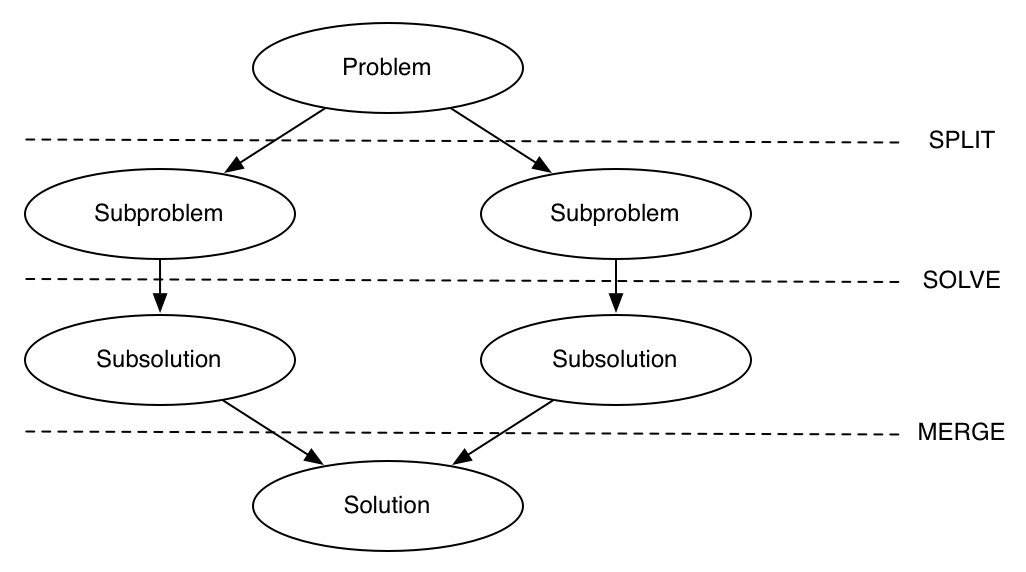
\includegraphics[width=\textwidth]{figsrc/DnC.png}
    \caption{A diagram showing how divide and conquer works.\label{fig:DnC}}
\end{figure}

\subsection{Main Contribution of This Dissertation}
\label{subsec:advantages}

\subsubsection{Reducing the Difficulty of Problems}

Due to characteristics of D\&C, all problems that can be accurately split are expected to be solved. For this dissertation, particularly, if the function detecting staves is reliable, then we can analyze arbitrarily complicated scores.

\subsubsection{Independence of Subproblems}

Typically, a score contains something useless for recognition such as the metadata of the song, lyrics, and even printed defects. By partitioning the original images into subimages where each contains only one staff, the amount of noisy information can be reduced and interference between staves is eliminated. Therefore, the detection tasks are independent between different staves.

\subsubsection{Parallelism}

Nowadays, a processor usually has multiple cores, and lots of computational tasks are implemented to be executed with parallel programs. In D\&C algorithm, the functions solving split subproblems are identically designed. With high independence and similar operations between subproblems, it is a good strategy to process them simultaneously. In other word, the original problem is suitable to be solved with \emph{SIMD (Single-Instruction-Multiple-Data)} parallel programs.

\chapter{Overview of OMR}
\label{c:overveiw-of-omr}

In this section, previous works of OMR are mentioned. Preprocessing (binarization, staff profiling, staff detection, and staff removal) and recognition (symbol segmentation, symbol classification) are included. 

\section{Binarization}

\if 0
\bibliography{thesis}
\graphicspath{{./figsrc/}}
\fi

In recognition of printed scores, the color information, namely R/G/B or R/G/B/A vectors, is not useful. Instead, only the intensity information is considered for recognition, so gray-scaled images are always used as the raw input. Furthermore, people always determine if each pixel is background (white) or foreground (black) in advance, and hence the binarization is included in most applications of OMR.

In Pinto's research~\cite{Pinto:2011:MSB}, two kinds of binarization methods were introduced depending on whether the binarization threshold is locally adjustable. The simplest way is applying a constant threshold to all pixels in the image, which is called \emph{global thresholding}. The global threshold can be obtained by finding a value that maximizes the variance~\cite{Otsu:1979:ATSMfGLH} between foreground and background pixels, preserves the most edge information~\cite{Chen:2008:ADTIBMboED}, or maximizes the similarity between the binarized image and the original image~\cite{Huang:1995:ITbMtMoF,Tsai:1995:AFTSPfMaUH}. However, it cannot be expected that the intensity in different small regions is constant over the document, and a constant threshold might not work at a different intensity level. In particular, near the boundary of a page in a book, the image might show a gradient-like difference in terms of the average intensity as compared to the region far from the book spine (Fig.~\ref{fig:bookspine}). To deal with such situations, the choice of the threshold should be determined by local information (nearby pixels)~\cite{Bernsen:2005:DToGLI}, which is called \emph{local thresholding}. In general, global thresholding is easier to be implemented, while local thresholding is more adaptive and robust.

\begin{figure}[ht]
    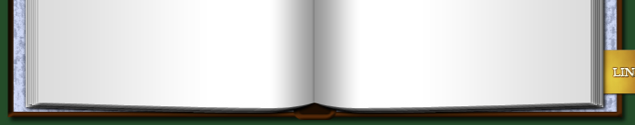
\includegraphics[width=\textwidth]{bookspine}
    \caption{Example of the gray-scale image near the book spine\label{fig:bookspine}.}
\end{figure}

\section{Staff Detection and Removal}

Dalitz et al.~\cite{Dalitz:2008:CSoSRA} introduced a systematic way for testing the staff removal algorithms. A dataset was generated from a set of ideal score images with the deformation methods listed in Table.~\ref{table:deformation}. The deformation algorithms and the CVC-MUSCIMA dataset are made openly available by Forns et al.~\cite{Forns:2012:CVC-MUSCIMA}.

\begin{table}[ht]
    %\hspace{-.5in}
    \begin{tabular}{|c|c|c|}
        \hline
        {\bf Deformation} & {\bf Type} & {\bf Parameter Description} \\
        \hline
        Curvature & deterministic & height/width ratio of sine curve \\
        \hline
        Typeset Emulation & both & \parbox[c]{9cm}{gap width, maximal height and variance of vertical shift} \\
        \hline
        Line Interruptions & random & \parbox[c]{9cm}{interruption frequency, maximal width and variance of gap width} \\
        \hline
        Thickness Variation & random & \parbox[c]{9cm}{Markov chain stationary distribution and inertia factor} \\
        \hline
        $y$-variation & random & \parbox[c]{9cm}{Markov chain stationary distribution and inertia factor} \\
        \hline
        Degradation & random & \parbox[c]{9cm}{emulating local distortions suggested by Kanungo et al.} \\
        \hline
        White Speckles & random & \parbox[c]{9cm}{speckle frequency, random walk length and smoothing factor} \\
        \hline
    \end{tabular}
    \caption{Deformation Methods\label{table:deformation}.}
\end{table}

% \input{discussion}
% \input{conclusion}

\appendix

\backmatter

\renewcommand{\bibname}{References}
\addcontentsline{toc}{chapter}{\bibname}
\bibliographystyle{ieeetr}

% Your bibliography goes here
{\singlespacing
\bibliography{thesis}
}

\end{document}
